\documentclass[/home/greg/Thesis/main/main.tex]{subfiles}

%\title{Neutron star mechanics in the observers inertial frame}
%\author{}

\begin{document}
\graphicspath{{/home/greg/Neutron_star_modelling/TimingNoiseModels/InertialSpaceResults/img/}}

\newcommand{\Jr}{J_{\textrm{rot}}}
\newcommand{\Ji}{J_{\textrm{in}}}

\section{Definitions}
In chapter \ref{sec: neutron star dynamics in the rotating frame} we
numerically solved Euler's rigid body equations in the rotating body frame
yielding the evolution of the spin vector $\spin$; this allowed us to observe
the dynamics such as precession and alignment without resolving individual
rotations. Physical observations of the star are made in the inertial frame and
so observers report on quantities calculable from the TOA of pulses. Generating
timing models for the phase, they quote results such as timing residuals and
the pulsation frequency and spindown. We aim to simulate these physical
observables and test the effect of various timing noise mechanisms. To do
this, we need to transform the solutions of Euler's rigid body equations into
observable quantities in the inertial frame. An efficient way to do this is to
determine the Euler angles which transform the rotating body frame axis,
denoted by $(x',y', z')$, to the inertial frame axis for which we will use $(x,
y, z)$. We will use the Euler angle parameterisation as described by
\citet{Landau1969}; a schematic of how these angles are constructed is given in
figure \ref{fig: Euler}. 
\begin{figure}[ht]
\centering
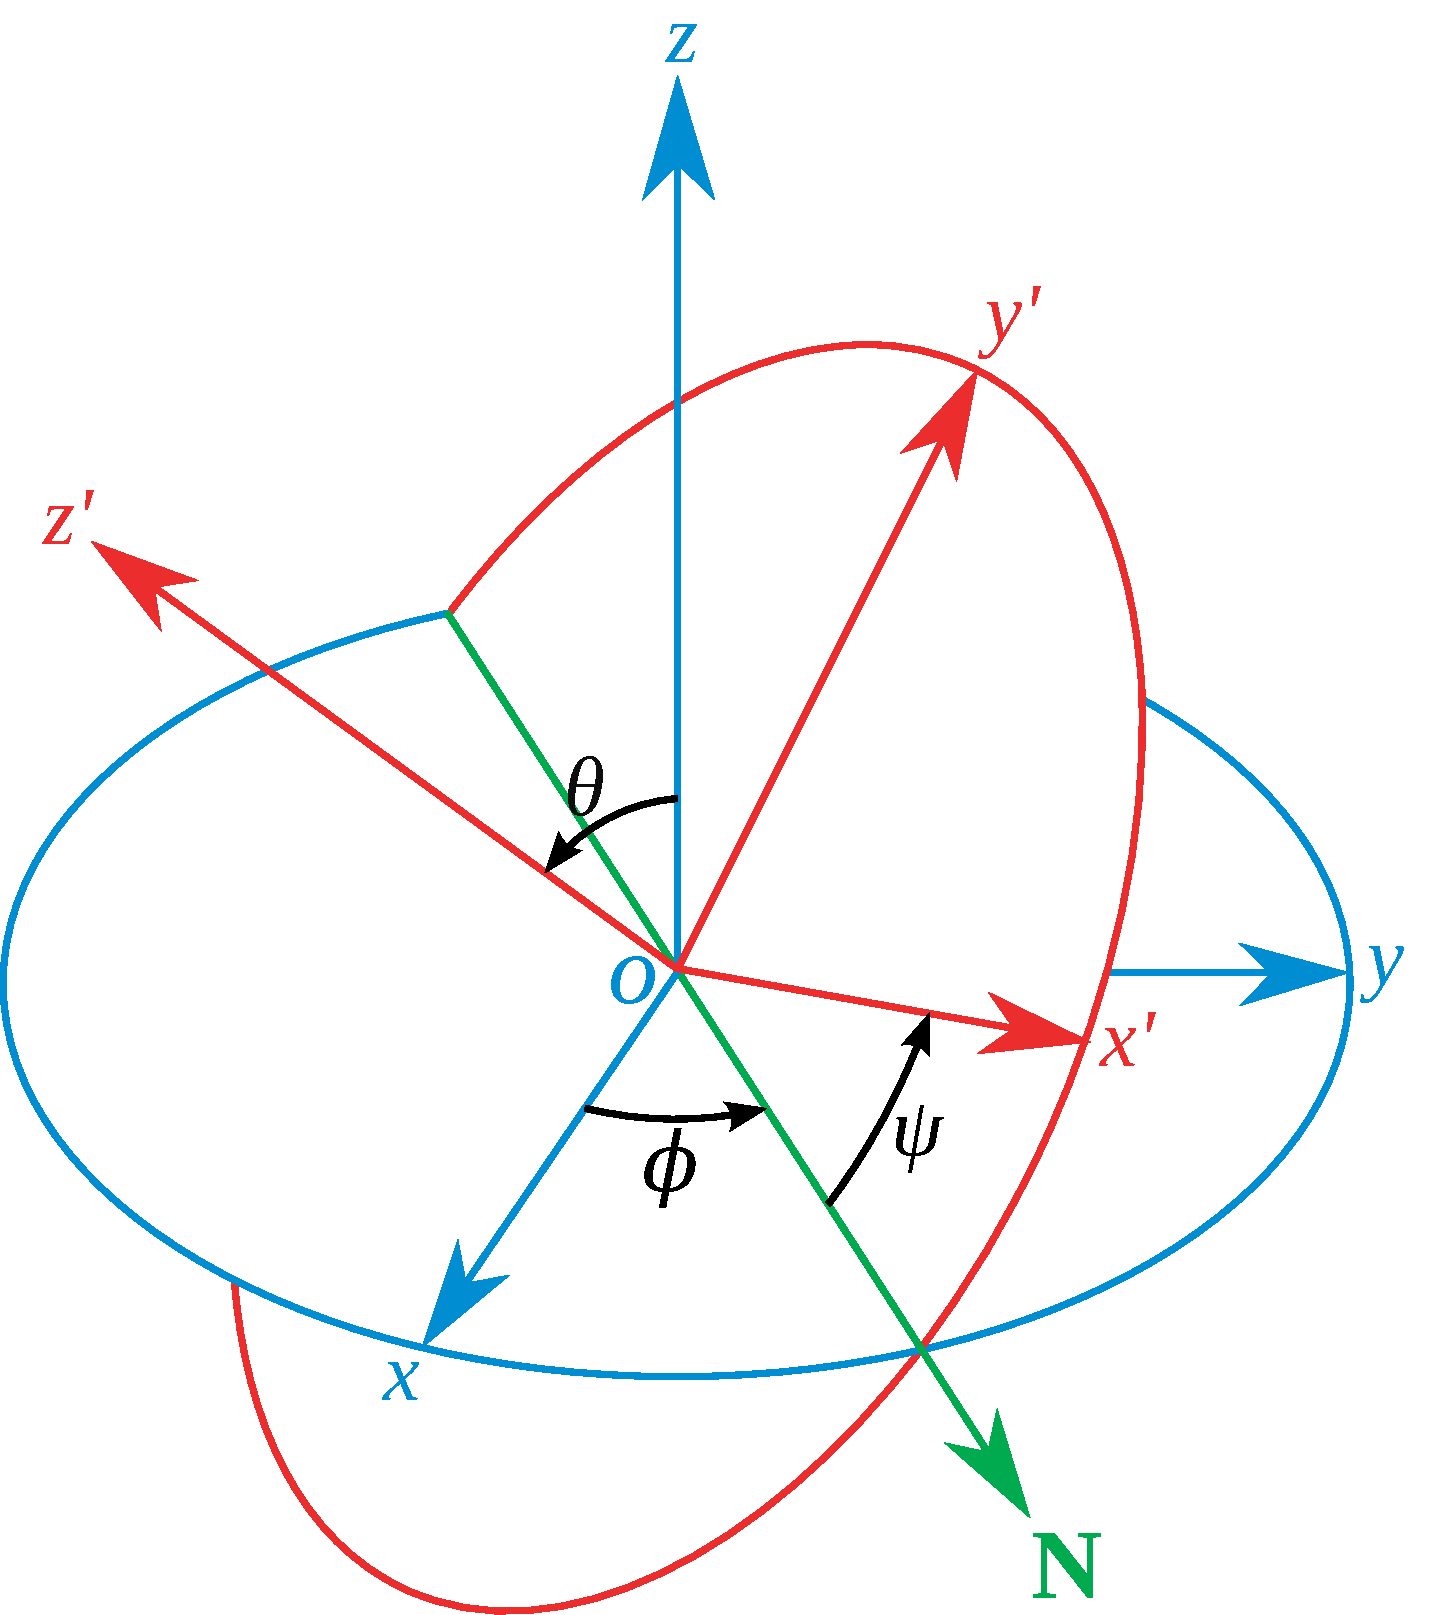
\includegraphics[scale=0.25]{Eulerangles-alternative.pdf}
% http://commons.wikimedia.org/wiki/File:Eulerangles-alternative.svg
\caption{Schematic of the Euler angle rotation. In the inertial frame the
angular momentum is set to lie initially along the $z$ axis. In the rotating
body frame for a biaxial body the deformation lies along $z'$ while the spin
vector initially lies along in the $x'- z'$ plane.}
\label{fig: Euler}
\end{figure}•

In the body frame, the diagonal moment of inertia tensor has components
$I_{xx}$, $I_{yy}$ and $I_{zz}$ and the star is spun down by a torque
$\boldsymbol{T}$. The Euler rigid body equations are then the left hand side
set of equations in \eqref{eqn: ODEs}. Decomposing the motion of the spin
vector into Euler angles and rearranging yields the right hand set of equations
in \eqref{eqn: ODEs}. These describe the evolution of the three Euler angles.
\begin{align*}
\dot{\omega_{x}} & = \frac{1}{I_{xx}}\left[T_{x} + 
                      \left(I_{yy} - I_{zz}\right) \omega_{y} \omega_{z}\right] 
& 
\dot{\theta} & = \omega_{x} \cos \psi - \omega_{y} \sin \psi
\\
\dot{\omega_{y}} & = \frac{1}{I_{yy}}\left[T_{y} + 
                      \left(I_{zz} - I_{xx}\right) \omega_{x} \omega_{z}\right] 
& 
\dot{\phi} & = \frac{\omega_{x} \sin \psi + \omega_{y} \cos \psi}{\sin \theta}
\numberthis \label{eqn: ODEs}
\\
\dot{\omega_{z}} & =\frac{1}{I_{zz}}\left[T_{z} + 
                      \left(I_{xx} - I_{yy}\right) \omega_{x} \omega_{y}\right]
& 
\dot{\psi} & = \omega_{z} - \dot{\phi} \cos \theta.
\end{align*}

These equations can be solved numerically using a time stepper, for now
we will use the rkf45 stepper provided by GSL. % Need reference
%The rotation period of the star is several orders of magnitude smaller than the
%precession period, as a result the Euler angles evolve on a much shorter time
%scale than the body frame spin components. This is numerically expensive. To
%allow efficient investigations we will therefore consider unrealistic values to
%understand the different types of motion before using realistic values only in
%cases of interest.

%Initially only torque free biaxial bodies are considered for simplicity, this
%system was studied by \citet{Jones2001} where it was demonstrated that for a
%biaxial body with deformation $\n_{d}$ along the $z'$ axis, this deformation,
%the spin vector and the angular momentum $\J$ are coplanar. They form a system
%which undergoes two different rotations: firstly at approximately the fast spin
%frequency the system rotates about $\J$ corresponding to a linear increase in
%$\phi$, then at the slower precession frequency the system counter rotates
%about $\n_{d}$ corresponding to a linear decrease in $\psi$ while $\theta$
%remains constant. This analytic example can be used to test the stability of
%numerical results before we go on to consider the effect of the torque and
%triaxiality. 

\section{Initial conditions}

Solving the rigid body equations in the body frame, we are free to impose the
following initial conditions on the spin vector
\begin{align}\label{eqn: spin init}
\omega_{x} & = \omega_{0}\sin(a_{0}), & 
\omega_{y} & = 0, & 
\omega_{z} & = \omega_{0}\cos(a_{0}),
\end{align}
such that $\spin(t=0)$ lies in the $x' - z'$ plane at an angle $a_{0}$ to the
$z'$ axis. For a well defined moment of
inertia and torque, this is sufficient to solve the rigid body equations. 

To define the transformation to the inertial frame, we use a rotation matrix 
$R(\theta, \phi, \psi)$ constructed from the Euler angles. Then the 
angular momentum vectors in the two frames are related by 
\begin{equation}
\Jr = R(\theta, \phi, \psi) \Ji .
\label{eqn: transform}
\end{equation}•
The angular momentum in the rotating frame has an initial condition 
set by 
\begin{equation}
  \Jr(t=0) = I \spin_0.
\end{equation}
If we set an initial condition on the angular momentum in the inertial frame,
we uniquely define the initial Euler angles. We are free to set the initial
angular momentum in the inertial frame to lie along the inertial $z$ axis such
that
\begin{equation}
  \Ji(t=0) = |J|\hat{z} 
\end{equation}
Normalising the two vectors in equation \eqref{eqn: transform} and rearranging
gives the expression 
\begin{equation}
\left[ \begin{array}{c}
\sin \psi_{0} \sin \theta_{0} \\
\sin \psi_{0} \cos \theta_{0} \\
\cos \theta_{0}
\end{array}\right]
 = \frac{1}{\sqrt{(I_{xx}\sin a_{0})^{2} + (I_{zz}\cos a_{0})^{2}}} 
\left[ \begin{array}{c}
I_{xx}\sin a_{0} \\
0 \\
I_{zz} \cos a_{0}
\end{array}\right].
\end{equation}•
We have three equations for two unknowns. Our choice to set $\J$ along
the $z$ axis leaves the initial value of $\phi$ a free variable; for simplicity
we set it by $\phi_{0} = 0$. Inserting this and comparing the components
\begin{equation}
\theta_{0} = \arccos\left(\frac{I_{zz}\cos a_{0}}{ \sqrt{(I_{xx}\sin
        a_{0})^{2} + (I_{zz}\cos a_{0})^{2}}} \right).
\label{eqn: theta init}
\end{equation} 
In the limit $\epsilon_{I} \ll 1$ we have that $\theta_{0} \approx a_{0}$.
For $\psi_0$, we can use that $\sin(\arccos(x)) = \sqrt{1 - x^{2}}$ giving:
\begin{equation}
\psi_0 = \frac{\pi}{2}.
\end{equation}
We now have a suitable set of initial conditions to solve the 6 ODEs in
\eqref{eqn: ODEs}.

\section{Biaxial body with no torque}

The precession of a spinning biaxial body free from torques can be described as
the superposition of two rotations.  The fast rotation due to the spin of the
star and a slower precession about the symmetry axis. Decomposing the motion
into the Euler angles \citet{Jones2001} demonstrated that: the wobble angle
$\theta$ remains fixed; the azimuthal angle $\phi$ monotonically increases at
the `spin frequency' $\dot{\phi}$; the body frame precession refers to the
decrease (for oblate bodies) of $\psi$ at the slower precession frequency
$\dot{\psi}$. So with the the initial conditions the analytic solutions take
the form
\begin{align}
    \theta(t) & = \theta_{0} \approx a_{0} \\
    \phi(t) & = \dot{\phi}t + \phi_{0} = \omega_{0} t \\
    \psi(t) & = \dot{\psi}t + \psi_{0}= -\epsilon_{I}\omega_{0}t+\frac{\pi}{2} 
    \label{eqn: euler angles torque free evolution}
\end{align}
We begin by testing that our numerical solutions of equations
\eqref{eqn: ODEs} is consistent with this description.

%we will now
%give a brief account of their results. Define two
%vectors: $\n_{J}$ which lies along the angular momentum vector and $\n_{d}$ which lies
%along the deformation axis, in this example this is the $z'$ axes.
%We can then decompose the angular velocity according to 
%\begin{equation}
%  \spin = \dot{\phi}\n_{J} + \dot{\psi}\n_{d}.
%\label{eqn: decomp}
%\end{equation}
%%The NS dynamics can then be described by the superposition of the two cones. 
%%The deformation axes $\n_{d}$ sweeps out a cone of half angle $\theta$ about
%%the $\n_{J}$ vector. Superimposed on this motion the $\n_{J}$ vector 
%we can show that $\phi$ monotonically increases at the fast spin frequency,
%$\psi$ decreases at the slower precession frequency whilst $\theta$
%remains constant. 

\subsection{Solving the equations}
In figure \ref{fig: biaxial body no torque} we present the solution of equation
\eqref{eqn: ODEs} for some typical values. In the left hand figure, the body
frame spherical components are given showing the usual torque-free precession.
In the right hand plot, we plot the Euler angles. This demonstrates `almost'
perfect agreement with \citetalias{Jones2001} for the Euler angles of a oblate
precessing body. That is, $\phi$ monotonically increases at the spin frequency
while $\psi$ decreases at the slower precession frequency. The polar angle
$\theta$ should remain constant during this simulation. Inspecting its value
however, we find it varies fractional level by $\sim 10^{-11}$.
This is caused by the finite numerical precision when calculating the
subtraction defined in equation \eqref{eqn: ODEs} for $\dot{\theta}=0$. On
short time scales these errors remain small and so
the results hold.  Over sufficiently long time scale these errors can
accumulate and eventually lead to a complete loss of numerical accuracy. We
must therefore be vigilant to ensure this does not occur when considering
realistic values.
\begin{figure}[ht]
    \centering
\subfloat[Spherical components in the body frame]
         {\includegraphics[width=0.7\textwidth]
         {{Spherical_Plot_chi0_80.00_omega0_1.00e+01_epsI3_1.00e-03_n_10000_a0_15.00_T_5.00e+03_upsilon_0.000_epsA_0.00e+00_epsI1_0.00e+00_AnomTorque_1}.pdf}} \\
\subfloat[Euler angles ]
         {\includegraphics[width=0.7\textwidth]
         {{Euler_Angles_chi0_80.00_omega0_1.00e+01_epsI3_1.00e-03_n_10000_a0_15.00_T_5.00e+03_upsilon_0.000_epsA_0.00e+00_epsI1_0.00e+00_AnomTorque_1}.pdf}}
\caption{Solution to the differential equations in \eqref{eqn: ODEs} for a
canonical biaxial NS with a deformation of $\epsilon_{I3} = 10^{-3}$. The red
dashed line is the analytic calculation found by \citet{Jones2001} for the
evolution of the Euler angles as given in equation 
\eqref{eqn: euler angles torque free evolution}.}
\label{fig: biaxial body no torque}
\end{figure}•

\FloatBarrier
%\paragraph{Convergence test}
%To ensure that the small wobble in $\theta$, which should remain constant, is
%a numerical effect rather than a lack of physics we can plot the fractional
%size of the wobble whilst changing the absolute error tolerance given to the
%ODE stepping procedure. This is done in figure \ref{fig: error}
% \begin{figure}[ht]
%\centering
%\includegraphics[scale=0.4]{error_plot.pdf}
%\caption{Fractional size of variations in theta plotted against the relative
%error tolerance given to the stepper.}
%\label{fig: error}
%\end{figure}
%We observe a strange behaviour in which the magnitude of the fractional difference, defined by
%\begin{equation}
%\textrm{Var}(\theta) = \frac{\theta_{\textrm{max}} - \theta_{\textrm{min}}}{|\theta|},
%\end{equation}
%increases exponentially as the error becomes very small. This is due to a
%change in the type of variation of theta, for larger absolute errors we
%observe a period wobble around the expected value of $\theta$. In contrast for
%much smaller absolute errors the solution seems to wander of the mean value
%whilst also undergoing a periodic wobble. We demonstrate this in figure
%\ref{fig: error example} for the two extremes values. 
%
%\begin{figure}[ht]
%\centering
%\includegraphics[scale=0.4]{error_example.pdf}
%\caption{Resulsts of simulations with different error tolerances,
%interestingly the smaller absolute error produces greater numerical
%inaccuracy.}
%\label{fig: error example}
%\end{figure}

\FloatBarrier

\subsection{Physical observables: dynamics of the magnetic dipole} 
Having the Euler angles allows us to transform from the rotating frame into the
inertial frame of an observer. Such an observer will measure the pulses from
the electromagnetic radiation that streams out along the open field lines of
the dipole $\m$ as the star rotates. In this model we will assume a thin
collimated beam is emitted along the magnetic dipole. In the body frame we
set $\m$ at an angle $\chi$ to the $z'$ axis with unit vector $[\sin(\chi), 0,
\cos(\chi)]$.  Using the Euler angles to transform to the inertial frame, the
components are given by
\begin{equation}
\m = 
\left[\begin{array}{c}
\cos\phi\cos\psi\sin\chi - \sin\phi \cos \theta \sin \psi \sin \chi 
+ \sin \phi \sin \theta \cos \chi \\
\sin\phi\cos\psi\sin\chi + \cos\phi \cos \theta \sin \psi \sin \chi 
- \cos \phi \sin \theta \cos \chi \\
\sin\theta \cos\psi \sin\chi + \cos\theta \cos \chi
\end{array}\right].
\label{eqn: m inertial}
\end{equation}•
Following the work of \citetalias{Jones2001} two angles $\Phi$ and $\Theta$ are
defined to describe the polar and azimuth of $\m$ in the inertial frame.
The azimuthal angle is given by 
\begin{equation}
    \Phi = \arctan\left(\frac{\m_{y}}{\m_{x}}\right) = 
\phi - \frac{\pi}{2} + \arctan\left(\frac{1}{\cos\theta}
                       \left(\frac{\cos\psi \tan \chi}{\tan\theta - 
                       \sin \psi \tan\chi }\right)\right),
\label{eqn: Phi}
\end{equation}
while the polar angle is
\begin{equation}
\Theta = \arccos(\m_{z}) = \arccos(\sin \theta \sin \psi \sin \chi + \cos \theta \cos \chi )
\label{eqn: Theta}
\end{equation}

Given a solution of equations \eqref{eqn: ODEs} we can use these two equations
to describe the evolution of the magnetic dipole orientation in the inertial
frame (its magnitude is assumed to be fixed). We will now go on to discuss how
this can be related to physical observables.

\subsubsection{Instantaneous electromagnetic frequency}

An observer sees a pulse from the NS every time the column from the magnetic
dipole passes through their location. For the frequency of pulsations, we are
interested only in the azimuthal evolution of the magnetic dipole. So we can 
simplify and say - a pulse
will occur every time the magnetic dipole cuts the plane containing the observer
and the angular momentum vector $\J$. We are neglecting the observers polar
position and assuming they do not sit along the spin axis.

Differentiating the phase with respect to time we have
\begin{equation}
\dot{\Phi} = \dot{\phi} 
+ \frac{\sin\chi \left(
\dot{\psi} (\cos\theta\sin\chi - \sin \psi \sin \theta \cos\chi) + 
\dot{\theta} \cos\psi (\cos\theta\sin\chi - \sin \psi \sin \theta \cos\chi)\right) 
}{(\sin\theta \cos \chi - \cos \theta \sin \psi \sin \chi)^{2} + \cos^{2}\psi \sin^{2} \chi}.
\label{eqn: Phi_dot}
\end{equation}•

This is then the \emph{instantaneous electromagnetic frequency}, an observer
will measure the time averaged value of $\dot{\Phi}$ as the `spin frequency' of
the star. Recalling that for a biaxial star with no torque $\theta$ is constant,
\citet{Jones2001} found the averaged frequency split into the cases 
$\theta > \chi$ and $\theta < \chi$.

\paragraph{Understanding the two cases}
To get a feeling for the mechanics we can decompose the rotation vector into 
rotations about the angular momentum and rotation about the deformation axis:
\begin{equation}
  \spin = \dot{\phi}\n_{J} + \dot{\psi}\n_{d}.
\label{eqn: decomp}
\end{equation}
Any fixed vector (such as $\m$) in the body frame can be understood in the
inertial frame as undergoing two motions: keeping $\phi$ fixed and increasing
$\psi$ rotates the vector in a cone about the $\n_{d}$ axis; holding instead
$\psi$ fixed and increasing $\phi$ sweeps the vector about a cone centred
around the $\n_{J}$ axis. Calling these cones the precession and spin cones
respectively the resulting motion can be understood as the superposition of the
two. \citetalias{Jones2001} found that the types of solutions these cones produced
depended on the ordering of $\theta$ and $\chi$. In figure \ref{fig: cones} an 
illustration is given of these cones
projected into the reference plane for the three possible orderings of $\theta$
and $\chi$. 

\begin{figure}[ht]
\centering
	\subfloat[$\theta > \chi$]{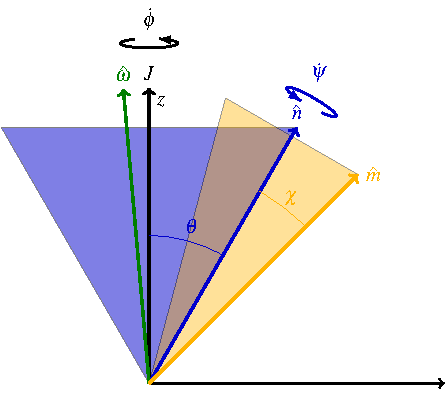
\includegraphics[width=0.33\textwidth]{chi_less_theta.pdf}}
	\subfloat[$\theta = \chi$]{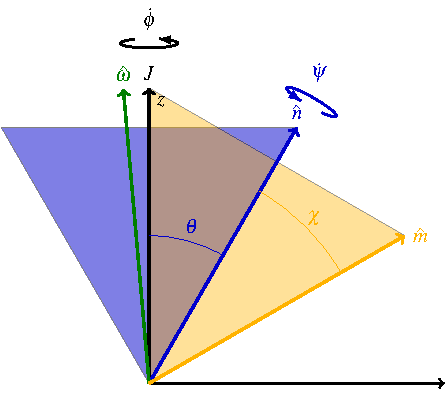
\includegraphics[width=0.33\textwidth]{chi_equal_theta.pdf}}
	\subfloat[$\theta < \chi$]{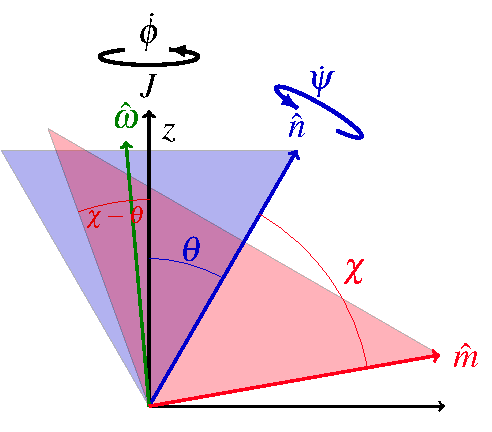
\includegraphics[width=0.33\textwidth]{chi_more_theta.pdf}}
\caption{Diagrams depicting 2D projections of the cones swept out by the
    different motions under torque free precession onto the reference plane.
    The yellow cone is swept out by the rotation of $\m$ about $\n_{d}$ at the
    slow precession frequency; the blue cone is swept out by the rotation of
    $\n_{d}$ about $\J$ at the fast spin frequency. The
precession cone rotates in the opposing direction to the spin cone for oblate
bodies.}
\label{fig: cones}
\end{figure}

The motion of the magnetic dipole about the precession cone evolves on a much
longer timescale than its motion about the spin cone; as a result the star will
always pulsate once every spin period, but the long precession will modulate
the average value on the precession timescale. Because of the large difference
in timescales, the motion of $\m$ can be considered as the slow evolution of a
third cone swept out by $\m$ about $\J$ which we will call the dipole cone. The
half angle made by this cone is exactly the polar angle $\Theta$ calculated
in equation \eqref{eqn: Theta}. The frequency with which $\m$ rotates around
dipole cone is given by equation \eqref{eqn: Phi_dot}. In figures \ref{fig:
variations}(a) and (b) the polar angle and frequency modulations are plotted for
three particular cases, with reference to these plots we now discuss the three
cases:

\begin{itemize}
\item The $\chi = \theta/2$ case: the precession cone is narrow and does not
extend over the angular momentum vector. The polar angle $\Theta$ of the dipole
cone oscillates periodically between $\theta+\chi$ and $\theta-\chi$
during a precession cycle. The spin frequency $\dot{\Phi}$ has an average value
of $\dot{\phi}$ and
oscillates about this value, comparing with the $\Theta$ variations
demonstrates these oscillations are locked in phase with the rotation of $\m$
in the precession cone. Recalling that the precession cone counter rotates with
respect to the spin cone, at $\theta+\chi$ the precession cone motion acts in
the opposing direction to the spin cone, this causes a reduction in the spin
frequency away from the average; by contrast at $\theta+\chi$ the counter
rotation is now in favour of the spin frequency and as a result the spin
frequency is increased above the average.

\item The $\chi = \theta$ case: here the angular momentum vector sits exactly
on the side of the precession cone, this suggest $\m$ can align exactly with
the angular momentum. When this happens the spin frequency tends to zero (due
to numerical error, this never actually occurs) manifesting as sharp dips in the
spin frequency; at the same time the polar angle tends to zero.

\item The $\chi = 4\theta$ case: The precession cone now extends over the
angular momentum vector, this means it always acts to reduce the spin
frequency; as a result the spin frequency has an average value of
$\dot{\phi} + \dot{\psi}$. The polar angle can vary between $\theta+\chi$ and
$\chi-\theta$, for $\chi$ close to $\theta$ the deviations away from the
average are large while as $\chi$ increases the deviations get smaller as
the half angle of the dipole cone increases.
\end{itemize}•

\begin{figure}[ht]
\centering
	\subfloat[Variations in polar angle]
  {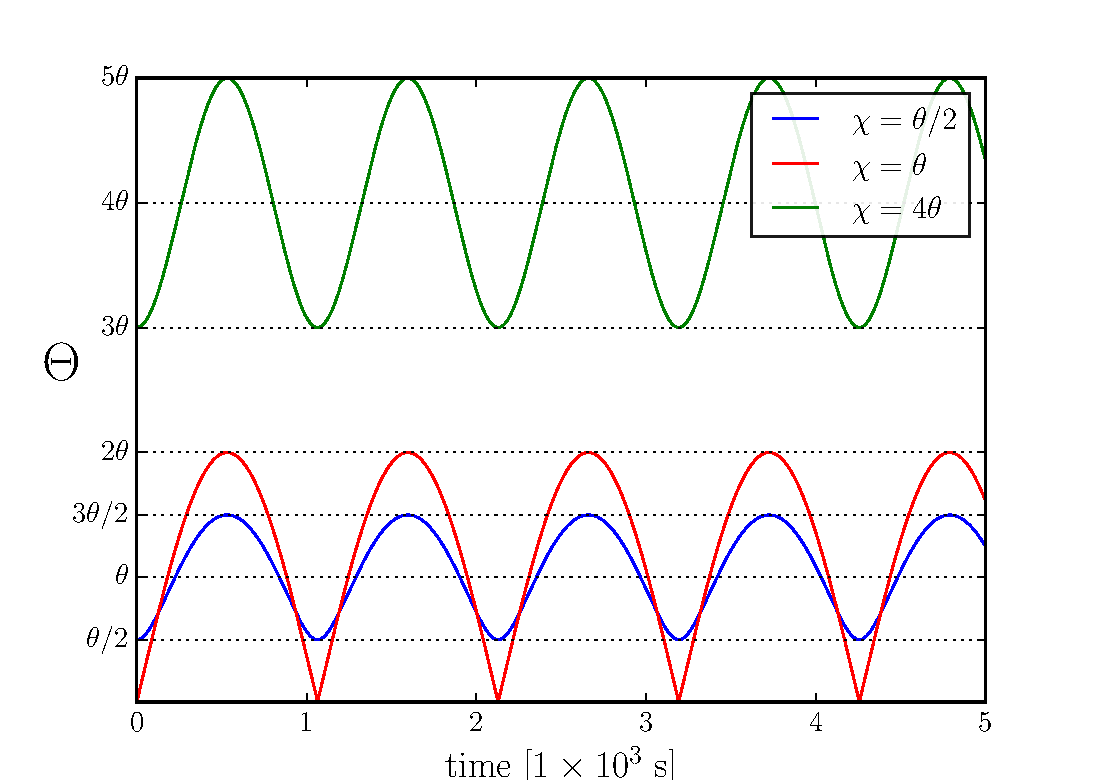
\includegraphics[width=0.7\textwidth]{polar_angle_variation_with_chi.pdf}}\\
	\subfloat[Variations in the spin frequency]
  {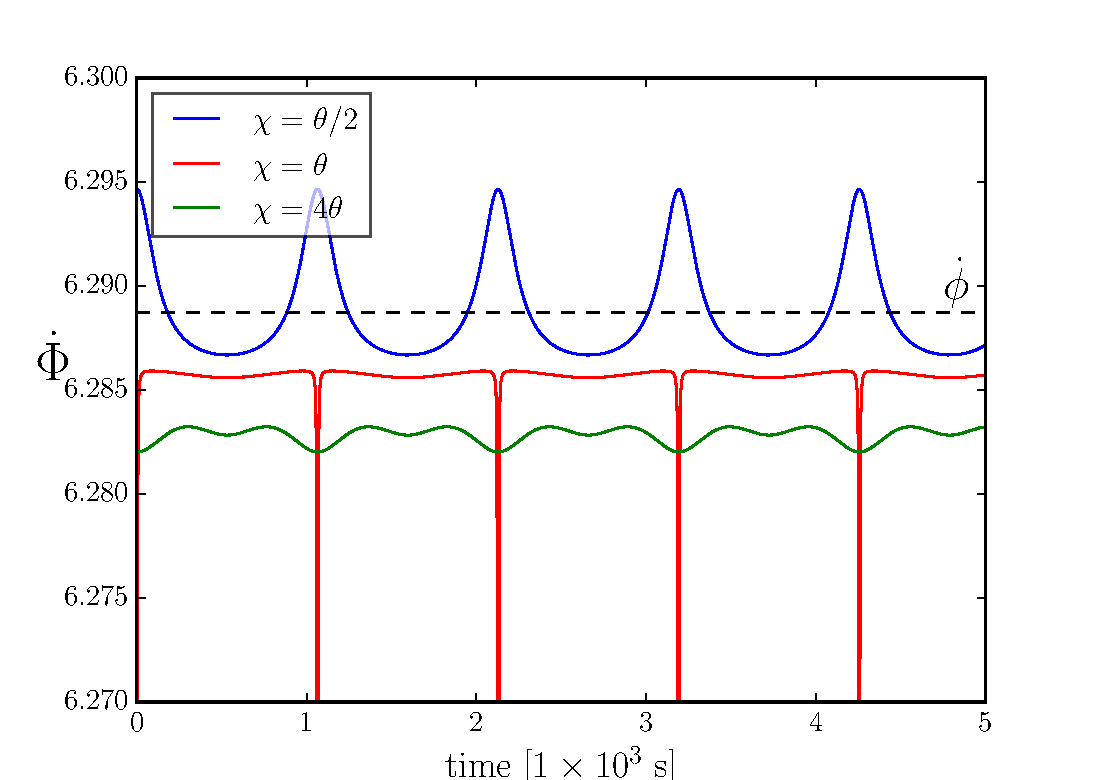
\includegraphics[width=0.7\textwidth]{frequency_variation_with_chi.pdf}} 
\caption{}
\label{fig: variations}
\end{figure}

\FloatBarrier
%\paragraph{Timing residuals}
%We now consider the timing residuals which would result from free precession
%alone. Clearly these are far from reality since the observed electromagnetic
%signal must act some torque on the body. Nevertheless, we can use equation
%\eqref{eqn: Phi} to calculate the exact phase of the signal. To compare with
%the tools used by observational astronomers we calculate the timing residual
%by fitting a third order Taylor series expansion to this phase. The residual
%is then the difference after subtraction
%
%\begin{figure}[ht]
%	\subfloat[$\chi<\theta$]{\includegraphics[width=0.5\textwidth]{{../../Timing_residuals/TR_chi_10.00}.png}}
%	\subfloat[$\chi > \theta$]{\includegraphics[width=0.5\textwidth]{{../../Timing_residuals/TR_chi_20.00}.png}}
%\caption{}
%\label{fig: }
%\end{figure}•

%\subsection{Biaxial body with torque}
%We now introduce the torque using the parameters of pulsar B1828-11 (Need to
%reference values here) to simulate a realistic pulsar making some assumptions
%on the cause of the periodic modulations. With realistic values the spin
%period is approximately a second, in comparison the precession period of the
%order of a year. The result is that we must resolve $10^{7}$ rotations of the
%neutron star per precessional orbit. 
%
%\begin{figure}[ht]
%	\subfloat[]{\includegraphics[width=0.5\textwidth]{{Spherical_Plot_chi_70.0_epsI1_0.00e+00_epsI3_9.37e-09_epsA_6.94e-12_omega0_15.51_aint_15_t1_3.00e+08}.pdf}}
%	\subfloat[]{\includegraphics[width=0.5\textwidth]{{Euler_Angles_chi_70.0_epsI1_0.00e+00_epsI3_9.37e-09_epsA_6.94e-12_omega0_15.51_aint_15_t1_3.00e+08}.pdf}}
%\caption{}
%\label{fig: }
%\end{figure}

\subsubsection{Timing residuals}

The principle indicator that a spin down power law does not accurately describe
the evolution of pulsars is the structure which exists in the timing
residuals. We now aim to introduce the tools required to calculate the timing
residuals from our model.

Equation \eqref{eqn: Phi} gives the exact phase evolution of the star, we will
label this as $\Phi_{\textrm{exact}}$. We then fit a Taylor expansion truncated
at the first order spin to $\Phi_{\textrm{exact}}$. The resulting coefficients,
$\dot{\nu}, \nu$ and $\phi_{0}$ are the physical quantities best describing the
NS under a power law spindown. Calculating the phase according to this Taylor
expansion gives $\Phi_{\textrm{fit}}$, the fitted phase. The residual is then
defined as the difference between these two
\begin{equation}
  \Delta\Phi = \Phi_{\textrm{exact}} - \Phi_{\textrm{fit}}
\end{equation}
In figure \ref{fig: TR no torque} we plot the timing residuals as calculated in
the torque free model for several values of $\chi$. It is worth noting that the
power law spin down assumes that the star is in fact spinning down; without the
torque this model can't not spin down. We can however interpret these results
as the effect of precession on timing residuals in the limit for which the
variation due to precession is much stronger than the spin down.
\begin{figure}[ht]
\centering
	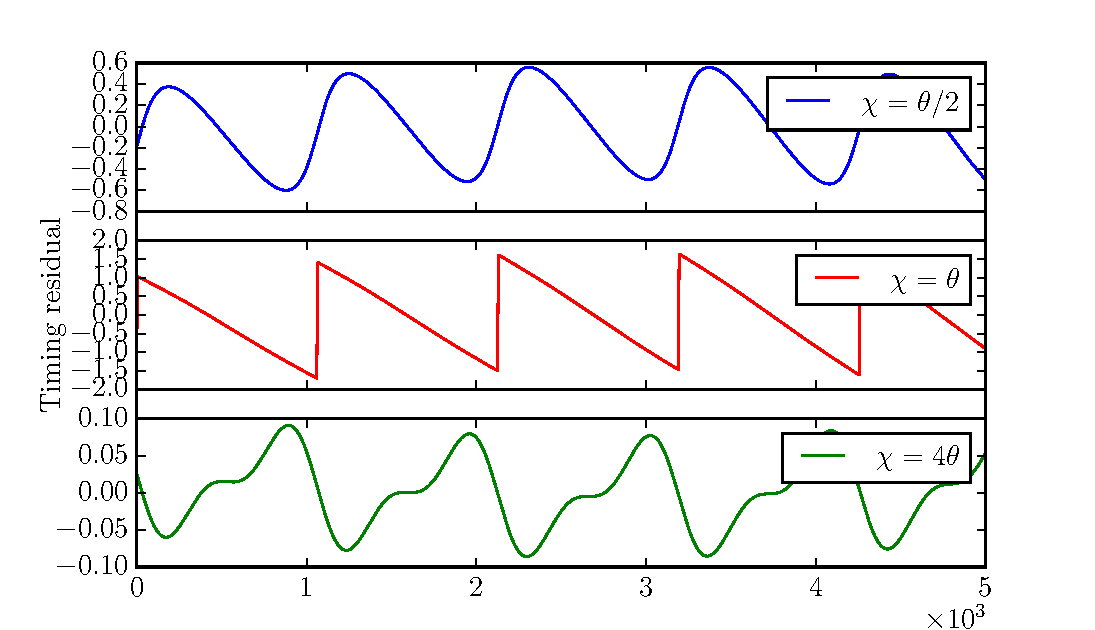
\includegraphics[width=0.7\textwidth]{Timing_residuals_no_torque.pdf}
\caption{Plot of the timing residuals for various angles of $\chi$ in the torque free model. }
\label{fig: TR no torque}
\end{figure}
The results show that the precession induces a periodic variation on the
precession timescale, the magnitude is proportional to the angle $\chi$. We 
also find the results are dependant on the initial angle $a_{0}$.

\subsubsection{Slowdown Rate $\dot{\nu}$}

The second observable which is often considered in characterising periodic
patterns in pulsar signals is the slowdown rate. In this simple model the
slowdown rate is given by $\ddot{\Phi}$, however calculating an analytic
expression is difficult, although theoretically possible. As an alternative, we
can use the method proposed by \citet{Lyne2010} to measure changes in the
spindown of observed pulsars. Second order Taylor expansions are fitted to
short sections of data of length $T$ and the resulting coefficient $\dot{\nu}$
is recorded. Repeating this process every $\sim T/4$ through the data set
builds picture of how the spindown varies with time. We choose $T$ such that it
is a fraction of the precession period over which we expect quantities to be
modulated.
\begin{figure}[ht]
\centering
	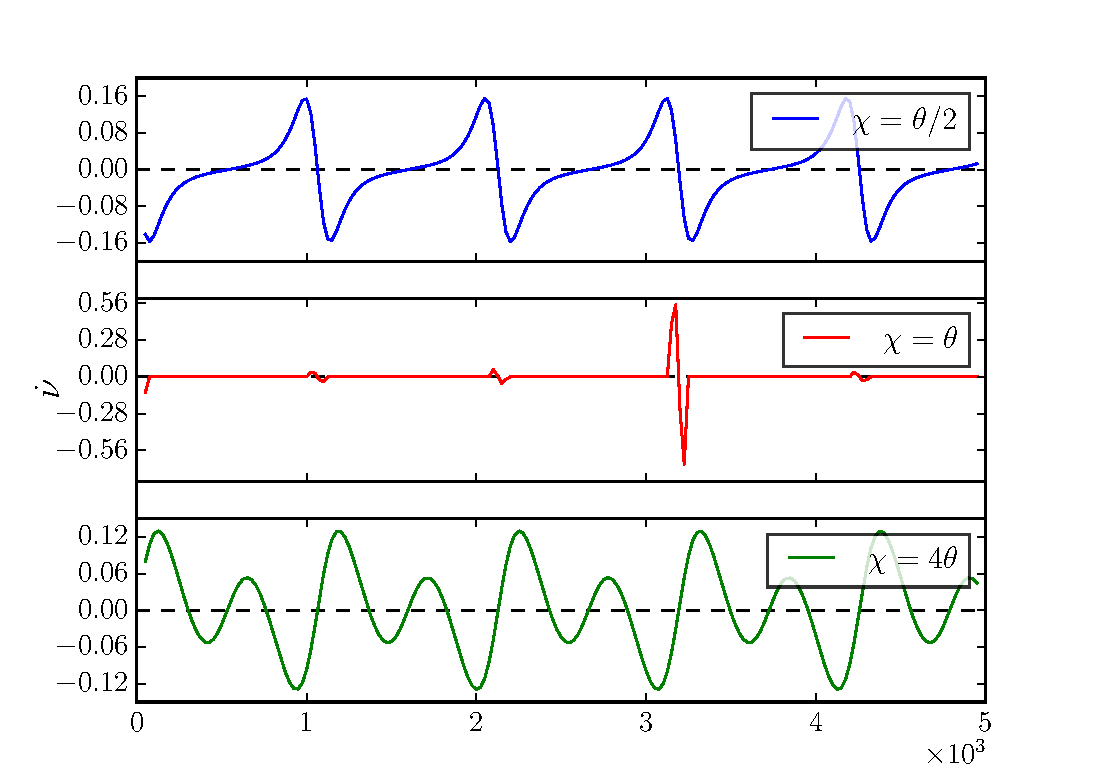
\includegraphics[width=0.9\textwidth]{nu_dot_no_torque.pdf}
\caption{Slow down rate }
\label{fig: nu_dot no torque}
\end{figure}

The variations seen in figure \ref{fig: nu_dot no torque} are the result of
free precession. As there is no torque, the overall spindown is zero. However,
due to precession the magnetic dipole performs a slow rotation about the
deformation axis. During half the cycle it counter-rotates and in the other
half it corotates with the rapid rotation about the angular momentum vector.
The result is a symmetric modulation of the spindown about zero. This
modulation depends upon the exact geometry. For the $\chi=\theta$ case the cone
lies exactly on the spin vector. As such their should be no variation in the
spindown. The observed spikes are numerical errors.

\subsubsection{Pulse amplitude}
Assuming a fixed magnitude of the magnetic dipole, the pulse amplitude will 
depend on the orientation of the magnetic dipole to the observer. It will be 
maximal when pointing directly at the observer and presumably fall off as the
angle between the two grows. To model this we take an observers position as 
$\Phi_{O}, \Theta_{O}$ and then assume the emission region follows
a two dimensional Gaussian:
\begin{equation}
A(\Phi, \Theta) = A_{0} \textrm{exp} \left(
                         -\frac{\tilde{\Phi}^{2}}{2\sigma_{\Phi}^{2}}
                         -\frac{\tilde{\Theta}^{2}}{2\sigma_{\Theta}^{2}}
                                     \right)
\label{eqn: Amplitude}
\end{equation}•
where $\tilde{\Phi}=\mod_{2\pi}(\Phi)-\Phi_{O}$ and 
$\tilde{\Theta}=\mod_{\pi}(\Theta) - \Theta_{O}$. Computing the angles $\Phi$ and $\Theta$ from numerical
solutions of the original ODEs and using the above emission model gives 
the pulse amplitude as seen be an observer. An example of a solution showing
the individual pulses along with the modulation due to free precession is
given in figure \ref{fig: amplitude_variation}
\begin{figure}[htb]
\centering
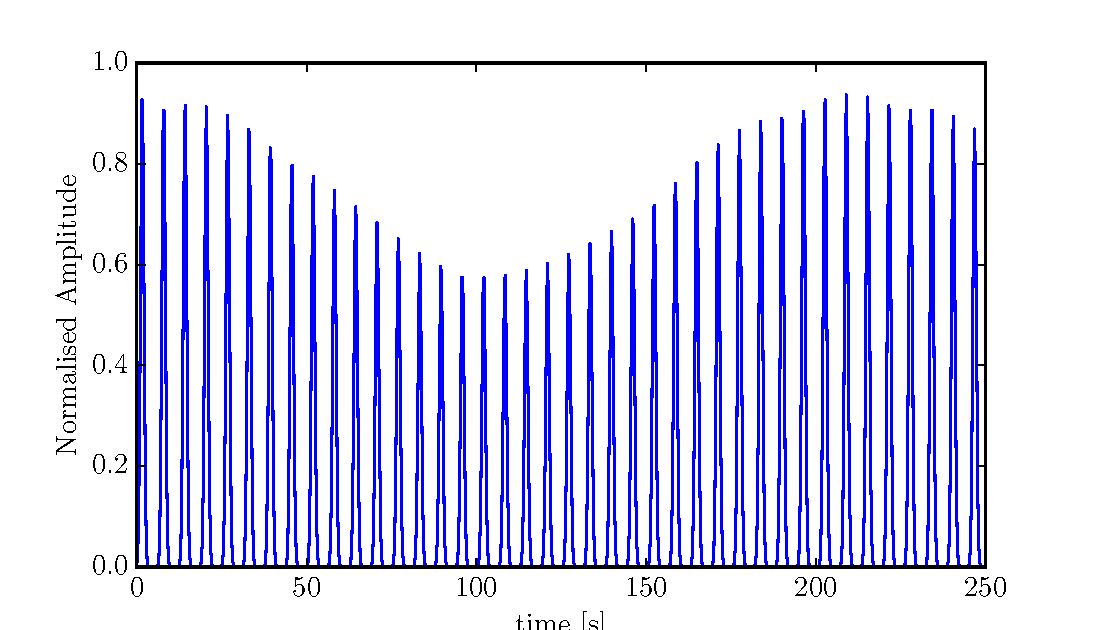
\includegraphics[width=.75\textwidth]{amplitude_variation}
\caption{Amplitude variation using a 2D Gaussian emission.}
\label{fig: amplitude_variation}
\end{figure}•

\FloatBarrier
\subsubsection{Pulse width}
The modulation of the amplitude coincides with modulations of the pulse width.
These have been measured with great accuracy by \citet{Lyne2010} and their
correlation with perceived changes in the spindown is key evidence for the two
state switching model. We can extract the pulse width analytically from
equation \eqref{eqn: Amplitude} by noting that $\Theta$ varies on the slow
precession timescale while $\Phi$ varies on the rapid spin timescale. We are
looking to measure the variations with respect to the slow precession timescale
so we can treat it as a constant. The full with at half maximum, corresponding
to the $W_{50}$ value of \citet{Lyne2010} occurs when
\begin{align}
A(\Phi, \Theta) = A_{0} \frac{1}{2} 
\end{align}
The condition for a full width half maximum at a fixed value of $\tilde{\Theta}$ 
is then
\begin{align}
\tilde{\Phi}_{50} = \pm\sigma_{\Phi}\left(\ln(2) 
          - \frac{\tilde{\Theta}}{\sigma_{\Theta}^{2}}\right)^{1/2}
\end{align}
If $P$ is the period of the rapid spin motion, then the fraction $W_{50}/P$
must be equal the fraction of the cycle spent above the full width half maximum
which is given by $2\tilde{\Phi}_{50} / 2\pi$. Writing this in terms of the
frequency $\dot{\Phi}$ rather than period we have
\begin{equation}
W_{50} = \frac{1}{\pi\dot\Phi}\sigma_{\Phi}\left(\ln(2) 
     - \frac{\tilde{\Theta}}{\sigma_{\Theta}^{2}}\right)^{1/2}
\label{eqn: pulse width}
\end{equation}•

In figure \ref{fig: PulseWidthModulation} we plot the pulse width as a function
of time for a canonical pulsar with $\chi=70^{\deg}$. 
\begin{figure}[ht]
\centering
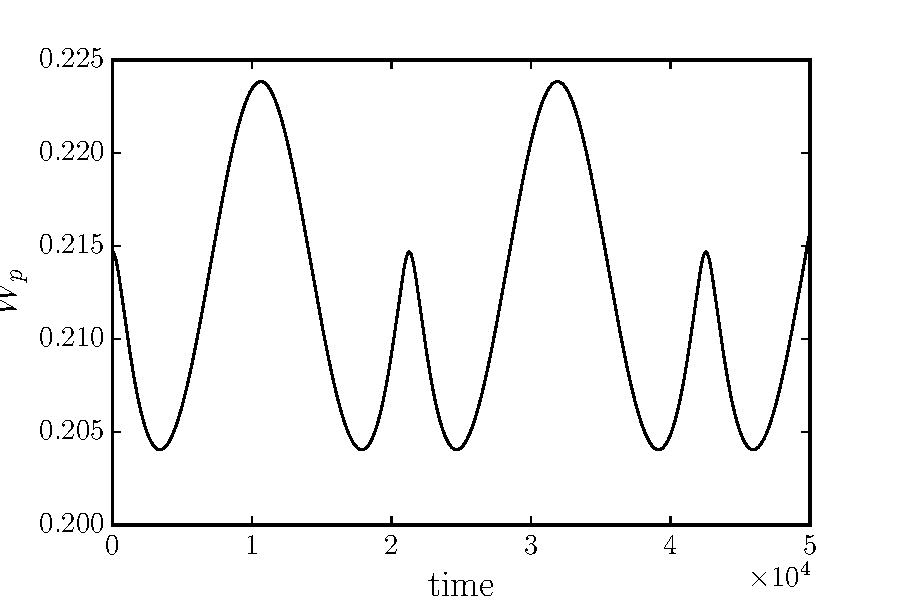
\includegraphics[width=.5\textwidth]{Pulse_width_modulation}
\caption{Pulse width as calculated by equation \eqref{eqn: pulse width} }
\label{fig: PulseWidthModulation}
\end{figure}•

\FloatBarrier

\section{Future work}
This work is currently incomplete. In the future we intend to:
\begin{itemize}
    \item Study how the observable properties described in this chapter change
      with the inclusion of the Deutsch torque.
      
   \item Compare the results of the previous item with pulsars which show evidence
   of free-precession such as B1828-11.

   \item Perform a Monte-Carlo study using the observables calculated in this chapter
   to generate a pulsar population similar to the observed population. The aim here
   would be to study the link between parts of the model (e.g. the anomalous torque, 
   the spin frequency, and non-sphericity) and the observed braking index. This can
   be calculated from the quantities described in this chapter. This would allow us
   to evaluate free-precession as a mechanism to explain the anomalous braking indices
   seen by \citet{Biryukov2012}.

   \item Include internal damping into the model; for example using the \citet{Bondi1955}
   model.

   \item Include torque switching based on the phase of free-precession. The aim here
   is to add a physical model to the two state switching proposed by \citet{Lyne2010}
   using the physics described by \citet{Jones2012}. 
\end{itemize}

%\section{Biaxial body with torque}
%We can now repeat the previous simulations but this time, include the torque.
%TBD
%The torque which produce the observed electromagnetic radiation will play an important role in determining the time variability of the observed pulse on earth. The torque is modelled as a magnetic dipole, denoted by $\m$, frozen into the star at an angle $\chi$ to the $z'$ axis in the $x'-z'$ plane. Following the work of \citet{Deutsch1955}, the torque is presented here in form found in \citet{Goldreich1970}.
%\begin{equation}
%\boldsymbol{T}=\frac{2R}{3c} I_{0}\epsilon_{A}\omega^{2}(\boldsymbol{\omega} \times \hat{\boldsymbol{m}})\times \hat{\boldsymbol{m}} + \epsilon_{A}I_{0}(\boldsymbol{\omega} \cdot \hat{\boldsymbol{m}})(\boldsymbol{\omega} \times \hat{\boldsymbol{m}}), \;\;\;\;\; \textrm{ with } \;\;\;\; \epsilon_{A} = \frac{m^{2}}{I_{0}R_{6}c^{2}},
%\label{eqn: torque}
%\end{equation}
%where $\boldsymbol{\omega}$ is the spin vector and $\epsilon_{A}$ is the magnetic deformation \citep[see][]{Glampedakis2010}.
%The first term on the right hand side is often referred to as the \emph{spin down}, or \emph{braking} torque. As this suggests it is responsible for the power law retardation of spin frequency and has an associated timescale $\tau_{S}$. The second term is known as the \emph{anomalous} torque which acts on a timescale $\tau_{A}$. Inserting this torque into the ODEs defined in \eqref{eqn: ODEs} then we have three time scales: the two due to the torque stated above and the precession time scale $\tau_{P}$ as found by \citet{Jones2001}. These three timescales are given by:
%\begin{align}
%\tau_{P} &= \frac{1}{\epsilon_{I}\nu_{0}}, & \tau_{A}&=\frac{1}{\epsilon_{A}\nu_{0}}, & \tau_{S}&=\frac{3c}{2R}\frac{1}{\epsilon_{A}\nu_{0}^{2}},
%\label{eqn: timescales}
%\end{align} 
%where $\nu_{0}$ is the initial spin frequency and $\epsilon_{I}$ is the magnitude of the elastic deformation along $z$ ($I_{zz} = I_{xx} + \epsilon_{I}$). In previous work we have shown % Maybe include this?
%that realistic NSs exist in the region $\tau_{P} > \tau_{A}$ for which $\epsilon_{A} < \epsilon_{I}$, in order to demonstrate the effect of the torque we will work for $\epsilon_{A} = \epsilon_{I}/2$. 
%\subsection{Results}
%In figure \ref{fig: biaxial body with torque} we plot the spherical components of the spin vector in the body frame (a), and the evolution of the Euler angles. Comparing this with figure \ref{fig: biaxial body no torque} the most striking difference is the wobble in both $\theta$ and $a$, on closer inspection one also finds this wobble in the other angles and the magnitude of $\spin$ along with a monotonic spin down.
%
%\begin{figure}[ht]
%	\subfloat[]{\includegraphics[width=0.5\textwidth]{{Spherical_Plot_chi0_80.00_omega0_1.00e+01_epsI3_1.00e-03_n_10000_a0_15.00_T_5.00e+03_upsilon_0.000_epsA_5.00e-04_epsI1_0.00e+00_AnomTorque_1}.pdf}}
%	\subfloat[]{\includegraphics[width=0.5\textwidth]{{Euler_Angles_chi0_80.00_omega0_1.00e+01_epsI3_1.00e-03_n_10000_a0_15.00_T_5.00e+03_upsilon_0.000_epsA_5.00e-04_epsI1_0.00e+00_AnomTorque_1}.pdf}}
%\caption{Solution to the differential equations in \eqref{eqn: ODEs} including the torque defined in \eqref{eqn: torque} for a biaxial body with $\epsilon_{A}=\epsilon_{I}/2$ }
%\label{fig: biaxial body with torque}
%\end{figure}•
%
%\FloatBarrier
%\subsection{Observables}
%In figure \ref{fig: variations with torque} we reproduce plots of figure \ref{fig: variations} with the addition of the torque. The torque introduces two additional effects: $\dot{\Phi}$ the instantaneous electromagnetic frequency decays slowly, this is caused by the spin down torque and is full agreement with what we expect; a fast sinusoidal oscillation in $\dot{\Phi}$ on the spin time scale, observable as a broadening of the line, is a result of the anomalous torque. As for the polar angle $\Theta$ the anomalous torque causes slight changes in the limits of the sinusoidal variation. Both the anomalous torque effects can be understood by realising that this effectively adds a triaxiality into the moment of inertia tensor. % needs more explanation
%
%\begin{figure}[ht]
%\centering
%	\subfloat[Variations in the spin frequency]{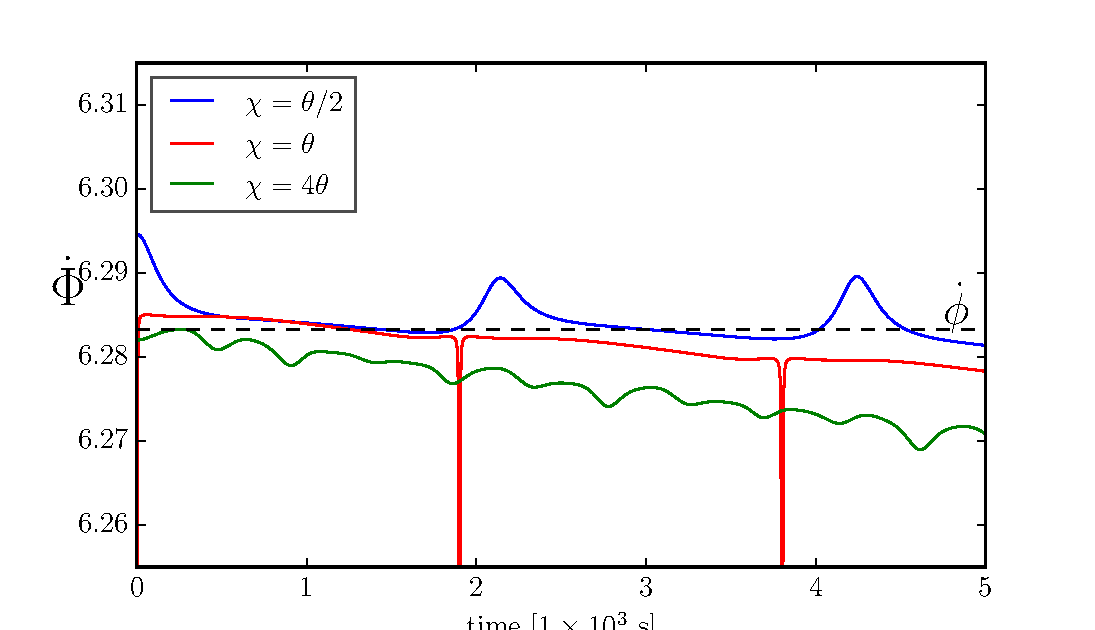
\includegraphics[width=0.7\textwidth]{frequency_variation_with_chi_inc_torque.pdf}} \\
%	\subfloat[Variations in polar angle]{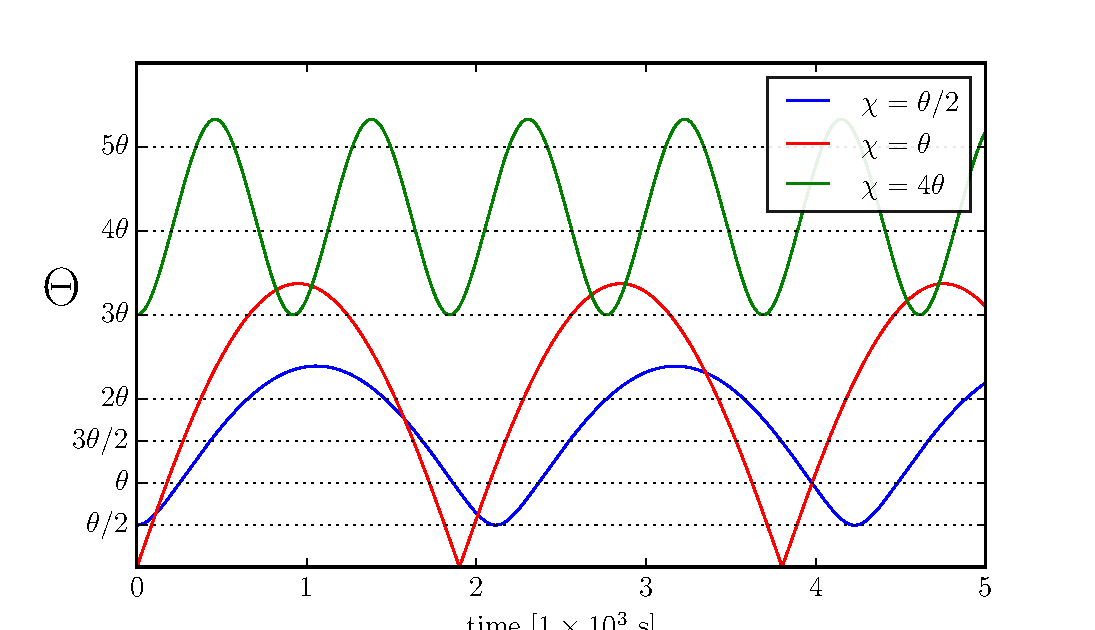
\includegraphics[width=0.7\textwidth]{polar_angle_variation_with_chi_inc_torque.pdf}}
%\caption{}
%\label{fig: variations with torque}
%\end{figure}
%
%\FloatBarrier
%\subsubsection{Timing residual}
%Including the torque the timing residuals are plotted in figure \ref{fig: TR with torque}, while the sinusoidal variation remains the magnetic inclination varies the spin down rate and hence the period of the these variations.
%\begin{figure}[ht]
%\centering
%	\subfloat[No anomalous torque ]{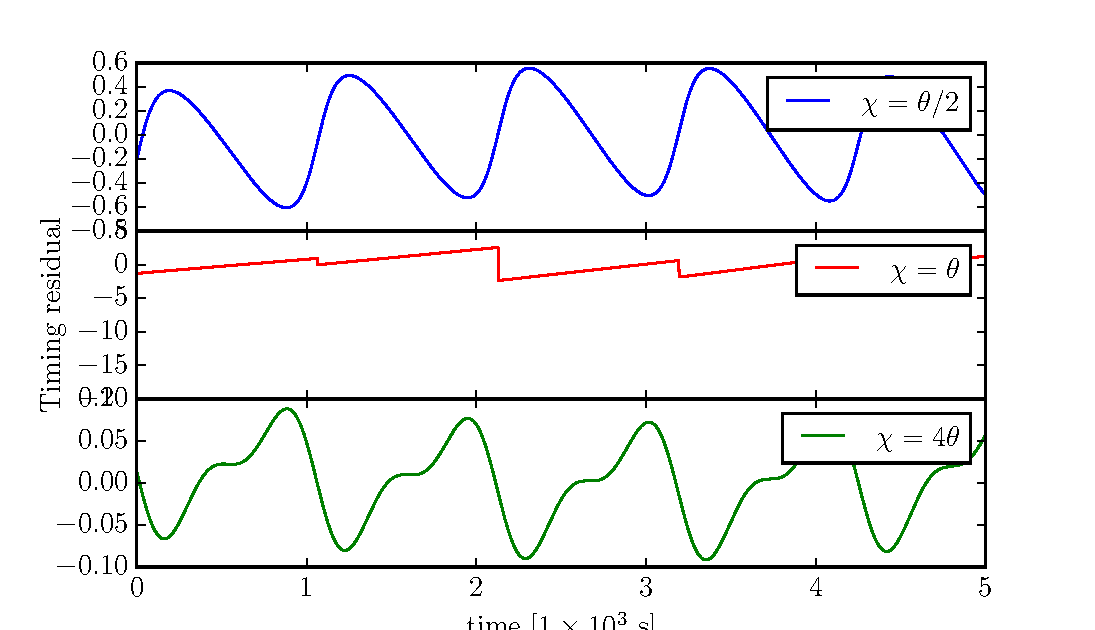
\includegraphics[width=0.6\textwidth]{Timing_residuals_with_torque_no_anom.pdf}} \\
%	\subfloat[With anomalous torque]{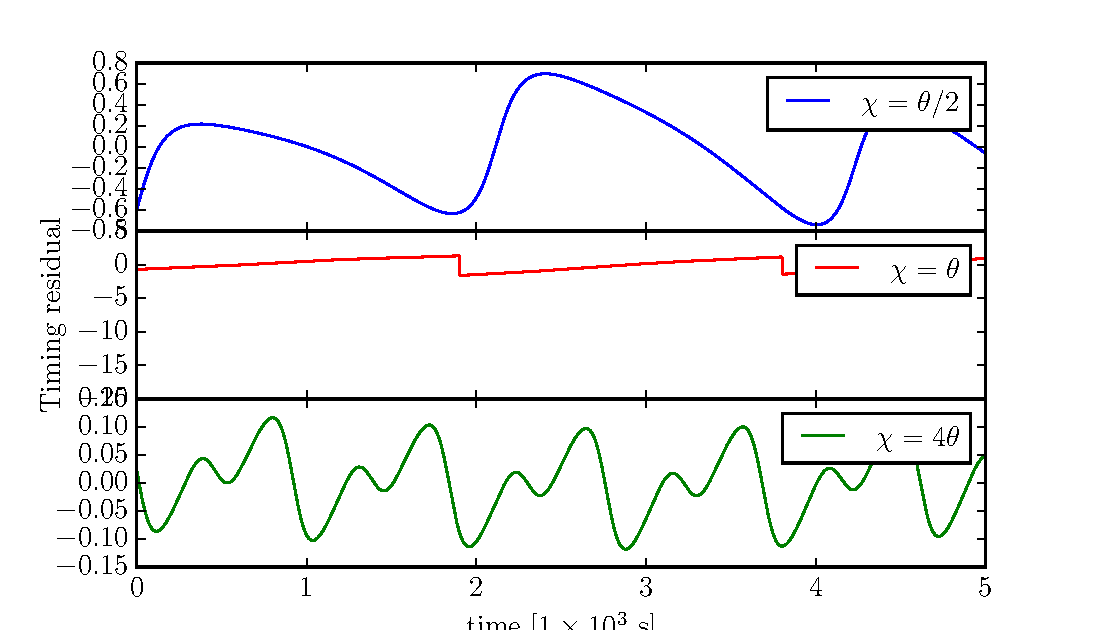
\includegraphics[width=0.6\textwidth]{Timing_residuals_with_torque.pdf}}
%
%\caption{Plot of the timing residuals for various angles of $\chi$ including the effects of the torque. }
%\label{fig: TR with torque}
%\end{figure}
%
%\FloatBarrier
%\subsubsection{Spindown Rate $\dot{\nu}$}
%The strength of the torque used in this model is parameterised by $\epsilon_{A}$ as given
%in equation \eqref{eqn: torque}. From \citet{Shapiro83} we can write this in terms of the
%magnetic field strength 
%\begin{equation}
%B_{s} = \frac{2m}{R^{3}}
%\end{equation}•
%Considering a simple model of a dipole at an angle $\alpha$ to the spin axis that characteristic
%age of NS can be defined as
%\begin{equation}
%t_{\textrm{ch}} = -\frac{\omega}{\dot{\omega}} = \frac{6 I_{0} c^{3}}{B_{s}^{2}R^{6} \sin(\alpha)^{2}\omega_{0}^{2}}
%\end{equation}
%Rearranging this expression to solve for the spindown rate yields
%\begin{align}
%\dot\omega = - \omega \frac{B_{s}^{2}R^{6} \sin(\alpha)^{2}\omega_{0}^{2}}{6I_{0}c^{3}}
%\end{align}•
%We can write this in terms of the torque deformation
%\begin{align}
%\dot\omega(t) = - \frac{2}{3}\omega(t) \sin^{2}(\alpha) \omega_{0}^{2} \frac{R}{c}
%\label{eqn: EM spindown}
%\end{align}
%
%Pulsars, except in rare cases corresponding to globular clusters, have strictly 
%negative spindown rates resulting from the electromagnetic torque and 
%the emmision of gravitional radiation. To be consistent with observations then
%we should constrain outselves to solutions for which the symmetric variations
%about the mean spindown as induced by free precession are smaller than the 
%spindown given in \eqref{eqn: EM spindown}. From \citet{Jones2001} we can
%consider a vacuum point-dipole spin-down torque so that
%\begin{equation}
%\ddot{\Phi} = k \dot{\Phi} \sin^{2}\Theta
%\end{equation}
%then departure from a non-precessing power-law spin-down may be written
%\begin{align}
%\frac{\Delta\ddot{\Phi}}{\ddot{\Phi}} = \left(3 \frac{\Delta\dot{\Phi}}{\dot{\Phi}} + \frac{\Delta(\sin^{2}\Theta)}{\sin^{2}\Theta}\right)
%\end{align}
%It can be shown that 
%\begin{align}
%\frac{\Delta\dot{\Phi}}{\dot{\Phi}} & \approx \frac{\cos(\chi)}{\sin(\chi)}\sin(\psi) \epsilon_{I}\theta, &&
%\frac{\Delta(\sin^{2}\Theta)}{\sin^{2}\Theta} \approx \frac{2\theta\sin\chi\cos\chi\sin\psi}{\sin^{2}\chi - 2\theta\sin\chi\cos\chi\sin\psi}
%\end{align}•
%
%\begin{figure}[ht]
%\centering
%	\subfloat[No anomalous torque ]{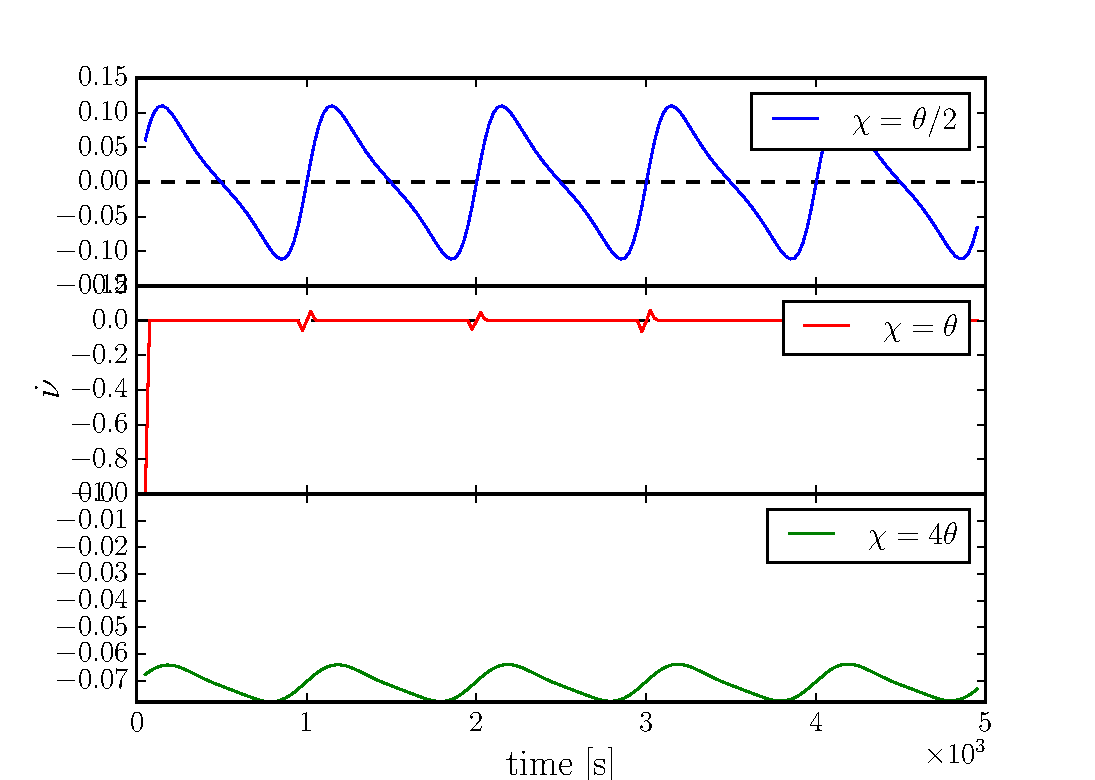
\includegraphics[width=0.6\textwidth]{nu_dot_with_torque_no_anom.pdf}} \\
%	\subfloat[With anomalous torque]{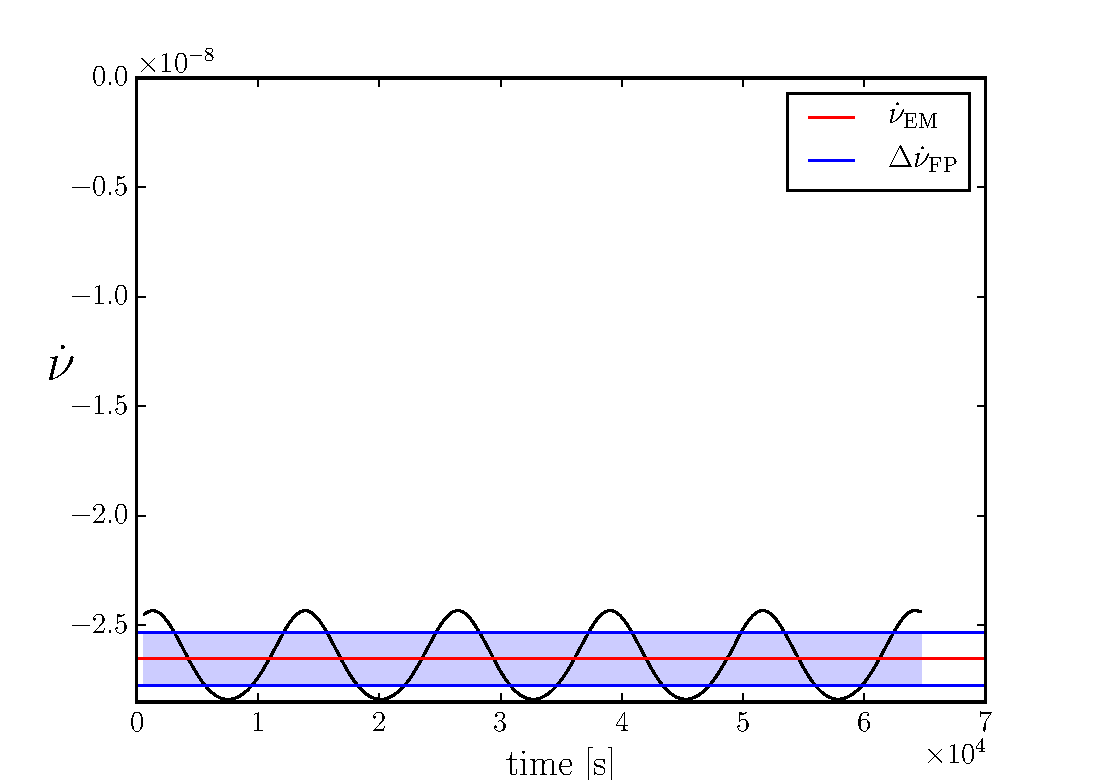
\includegraphics[width=0.6\textwidth]{nu_dot_with_torque.pdf}}
%\caption{}
%\label{fig: nu_dot no torque}
%\end{figure}
%
%\FloatBarrier
%
%\subsubsection{Pulse amplitude}
%
%\subsubsection{Pulse width}
%
%
%\FloatBarrier
%\section{B1828-11}
%In order to compare the prediction of our model with actual observations we select the pulsar B1828-11. There is some evidence in work by \cite{Lyne2000} that this pulsar undergoes precession, and work by \cite{Hobbs2010} and \cite{Lyne2010} documents the timing residuals and spin down rate with unsurpassed accuracy. This makes the pulsar ideal for study under the assumption that the variations are caused by precession.
%
%From table 1 in \citet{Lyne2000} we have that B1828-11 has a spin period of $P_{0}=405$ms. We can calculate the magnetic deformation using the surface magnetic field 
%\begin{equation}
%\epsilon_{A}=\frac{m^{2}}{I_{0}Rc^{2}}=\frac{(\frac{1}{2}B_{s}R^{3})^{2}}{I_{0}Rc^{2}}
%\end{equation}
%From table1 we have that $B_{s}=5\times10^{12}$G and using canonical values of $R$, $c$ and $I_{0}$\footnote{Should I give the actual values?} yields $\epsilon_{A}=6.94\times10^{-12}$.
%
%For the elastic deformations we have an upper limit from gravitational wave searches of $1\times10^{-6}$. We now make the assumption that it is precession which causes the variations in signal, from \citet{Jones2001} we may therefore use that 
%\begin{equation}
%\epsilon_{I} \sim \frac{P_{\textrm{spin}}}{P_{\textrm{precession}}}
%\end{equation}•
%Lyne found timescales of 1000, 500 and 250 days for the variations, we will use the shortest of these such that $P_{precession}=250$ days. Hence we have an elastic deformations of $1.88 \times10^{-8}$. This also agrees well with \citet{Lyne2010} B1812-11 is observed for $\sim6000$ days during which 22 oscillations occur, this gives a period of about $273$ days. 
%With these values we have the following timescales
%\begin{equation*}
%\tau_{S}=1.06\times10^{15} \textrm{ s} \;\;\;\; \;\;\;\; \tau_{A}=5.83\times10^{10} \textrm{ s} \;\;\;\; \;\;\;\; \tau_{P}=3.55\times10^{6} \textrm{ s}
%\end{equation*}•
%
%No obvious way exists to define $\chi$ other than to assume it must not be aligned on grounds that we can observe the pulsar. Since this pulsar satisfies the region A conditions and is therefore subject to the critical of $\chi$ we again choose the two values of $\chi$ previously used.

\biblio
\end{document}

